% Copyright (c) 2022 by Lars Spreng
% This work is licensed under the Creative Commons Attribution 4.0 International License. 
% To view a copy of this license, visit http://creativecommons.org/licenses/by/4.0/ or send a letter to Creative Commons, PO Box 1866, Mountain View, CA 94042, USA.

%~~~~~~~~~~~~~~~~~~~~~~~~~~~~~~~~~~~~~~~~~~~~~~~~~~~~~~~~~~~~~~~~~~~~~~~~~~~~~~
% You can add your packages and commands to the loadslides.tex file. 
% The files in the folder "styles" can be modified to change the layout and design of your slides.
% I have included examples on how to use the template below. 
% Some of it these examples are taken from the Metropolis template.
%~~~~~~~~~~~~~~~~~~~~~~~~~~~~~~~~~~~~~~~~~~~~~~~~~~~~~~~~~~~~~~~~~~~~~~~~~~~~~~


\documentclass[
11pt,notheorems,hyperref={pdfauthor=Maghfira Ramadhani}
]{beamer}


% Copyright (c) 2022 by Lars Spreng
% This work is licensed under the Creative Commons Attribution 4.0 International License. 
% To view a copy of this license, visit http://creativecommons.org/licenses/by/4.0/ or send a letter to Creative Commons, PO Box 1866, Mountain View, CA 94042, USA.

%~~~~~~~~~~~~~~~~~~~~~~~~~~~~~~~~~~~~~~~~~~~~~~~~~~~~~~~~~~~~~~~~~~~~~~~~~~~~~~
% Add your packages and commands to this file
%~~~~~~~~~~~~~~~~~~~~~~~~~~~~~~~~~~~~~~~~~~~~~~~~~~~~~~~~~~~~~~~~~~~~~~~~~~~~~~

%~~~~~~~~~~~~~~~~~~~~~~~~~~~~~~~~~~~~~~~~~~~~~~~~~~~~~~~~~~~~~~~~~~~~~~~~~~~~~~
\RequirePackage{palatino}
\RequirePackage[utf8]{inputenc}
\RequirePackage[T1]{fontenc}

\usefonttheme{serif}

\usepackage{styles/elegantmacros}
\usefolder{styles}
\usetheme[style=blue]{elegant}

\newcommand{\makepart}[1]{ % For convenience
\part{#1} \frame{\partpage}
}

%~~~~~~~~~~~~~~~~~~~~~~~~~~~~~~~~~~~~~~~~~~~~~~~~~~~~~~~~~~~~~~~~~~~~~~~~~~~~~~

%~~~~~~~~~~~~~~~~~~~~~~~~~~~~~~~~~~~~~~~~~~~~~~~~~~~~~~~~~~~~~~~~~~~~~~~~~~~~~~
% Figures
\RequirePackage{booktabs}
\RequirePackage{colortbl}
\RequirePackage{ragged2e}
\RequirePackage{schemabloc}
%\RequirePackage{natbib}
\RequirePackage{caption}
\RequirePackage{subcaption}
\RequirePackage{tabularx}
\RequirePackage{array}
\RequirePackage{multirow}
\usepackage[
  style=authoryear, 
]{biblatex}
\addbibresource{references.bib}
\newcolumntype{Y}{>{\centering\arraybackslash}X}

%~~~~~~~~~~~~~~~~~~~~~~~~~~~~~~~~~~~~~~~~~~~~~~~~~~~~~~~~~~~~~~~~~~~~~~~~~~~~~~

%~~~~~~~~~~~~~~~~~~~~~~~~~~~~~~~~~~~~~~~~~~~~~~~~~~~~~~~~~~~~~~~~~~~~~~~~~~~~~~
% Figures
\RequirePackage{wrapfig}
\RequirePackage{pgfplots}
\RequirePackage{graphicx}
\RequirePackage{adjustbox}
\RequirePackage{environ}
\pgfplotsset{compat=1.18}

\makeatletter
\newsavebox{\measure@tikzpicture}
\NewEnviron{scaletikzpicturetowidth}[1]{%
  \def\tikz@width{#1}%
  \def\tikzscale{1}\begin{lrbox}{\measure@tikzpicture}%
  \BODY
  \end{lrbox}%
  \pgfmathparse{#1/\wd\measure@tikzpicture}%
  \edef\tikzscale{\pgfmathresult}%
  \BODY
}
\makeatother
%~~~~~~~~~~~~~~~~~~~~~~~~~~~~~~~~~~~~~~~~~~~~~~~~~~~~~~~~~~~~~~~~~~~~~~~~~~~~~~

%~~~~~~~~~~~~~~~~~~~~~~~~~~~~~~~~~~~~~~~~~~~~~~~~~~~~~~~~~~~~~~~~~~~~~~~~~~~~~~
% Maths 
\RequirePackage{textcomp}
\RequirePackage{amsmath} 
\RequirePackage{amsthm}
\RequirePackage{mathtools}
%\RequirePackage{bbm}
%\RequirePackage{algorithm}
%\RequirePackage[osf,sc]{mathpazo}
%\RequirePackage{pifont}
%\newcommand{\xmark}{\ding{55}}%
%\numberwithin{equation}{section}
\DeclareMathOperator*{\argmax}{arg\,max}
\DeclareMathOperator*{\argmin}{arg\,min}

\setbeamertemplate{theorems}[numbered] % to number

\theoremstyle{definition}
\newtheorem{fact}{Fact}[section]
\newtheorem{examp}{Example}[section]

\theoremstyle{plain}
\newtheorem{definition}{Definition}[section]
\newtheorem{proposition}{Proposition}
\newtheorem{theorem}{Theorem}
\newtheorem{assumption}{Assumption}

\providecommand{\H}{\mathscr{H}}      
\providecommand{\E}{\mathbb{E}}
\makeatletter
\def\munderbar#1{\underline{\sbox\tw@{$#1$}\dp\tw@\z@\box\tw@}}
\makeatother

%~~~~~~~~~~~~~~~~~~~~~~~~~~~~~~~~~~~~~~~~~~~~~~~~~~~~~~~~~~~~~~~~~~~~~~~~~~~~~~
 % Loads packages and some defined commands

%% Pictograms

\def\up{\textuparrow\,}
\def\down{\textdownarrow\,}
\def\flat{\textrightarrow\,}
\def\then{$\rightsquigarrow\,$}
\def\so{{$\Rightarrow\,$}}
\def\tb{\textbar{}\,}
\newcommand{\al}[1]{\textbf{\alert{#1}}}
\newcommand{\alb}[1]{\textbf{\textcolor{blue}{#1}}}
\newcommand{\alg}[1]{\textbf{\textcolor{teal}{#1}}}
\newcommand{\alr}[1]{\textbf{\textcolor{red}{#1}}}

\title[
% Text entered here will appear in the bottom middle
]{Improving Rural Accessibility in Indonesia: Fuel Subsidy versus Infrastructure Development}

\author[
% Text entered here will appear in the bottom left corner
]{
    Maghfira Ramadhani 
}

\institute{
    School of Economics, \\
    Georgia Institute of Technology}
\date{\today}

\begin{document}

% Generate title page
{
\setbeamertemplate{footline}{} 
\begin{frame}
  \titlepage
\end{frame}
}
\addtocounter{framenumber}{-1}

% You can declare different parts as a parentof sections
\begin{frame}{Table of Contents}
    \tableofcontents%[part=1]
\end{frame}

%\makepart{Proposal}

\section{Introduction}
\begin{frame}
\begin{itemize}
    \item infrastructure \up \so cost \up \citeauthor{hartojo_2022}
    \item I created Elegant Slides because I wasn't satisfied with any of the existing Beamer templates, which look slightly different than Elegant Slides.
    \item My goal was to create a layout that is \al{simplistic but beautiful} and focuses on the content, rather than crowding each slide with lots of different coloured boxes.
    \item I designed Elegant Slides for \al{lecture notes and technical presentations} but it can be used for any kind of talk. 
\end{itemize}
\end{frame}

\subsection{Related Literature}
\begin{frame}
    Unless the user enters their own custom frame titles and subtitles, Elegant Slides automatically inserts the section title and, if specified, the subsection title as frame titles and frame subtitles.
\end{frame}

\section{Conceptual Framework}
\subsection{Accessibility in rural area}
\begin{frame}
\begin{itemize}
    \item Developing countries have been focusing on decentralization and local government reform with the believe that they are \alert{\textbf{more efficient}} in bringing local development (\cite{vazquez_2017}) 
    \item 
    \item 
\end{itemize}
\end{frame}

\subsection{Transportation structure in rural area}
\begin{frame}
\begin{itemize}
    \item Developing countries have been focusing on decentralization and local government reform with the believe that they are \alert{\textbf{more efficient}} in bringing local development (\cite{vazquez_2017}) 
    \item 
    \item 
\end{itemize}
\end{frame}

\section{Institutional Context and Background}
\subsection{Fossil fuel subsidy regime}
\begin{frame}
    This frame has a custom title and a custom subtitle.\footnote{This is a footnote. See also \textcite{hartojo_2022}. }
\end{frame}

\subsection{Decentralization of development}
\begin{frame}
    This frame has a custom title and a custom subtitle.\footnote{This is a footnote. See also \textcite{hartojo_2022}. }
\end{frame}


\begin{frame}
    \begin{figure}[t]
    \subcaptionbox{Village status in 2014\label{f:panel1}}{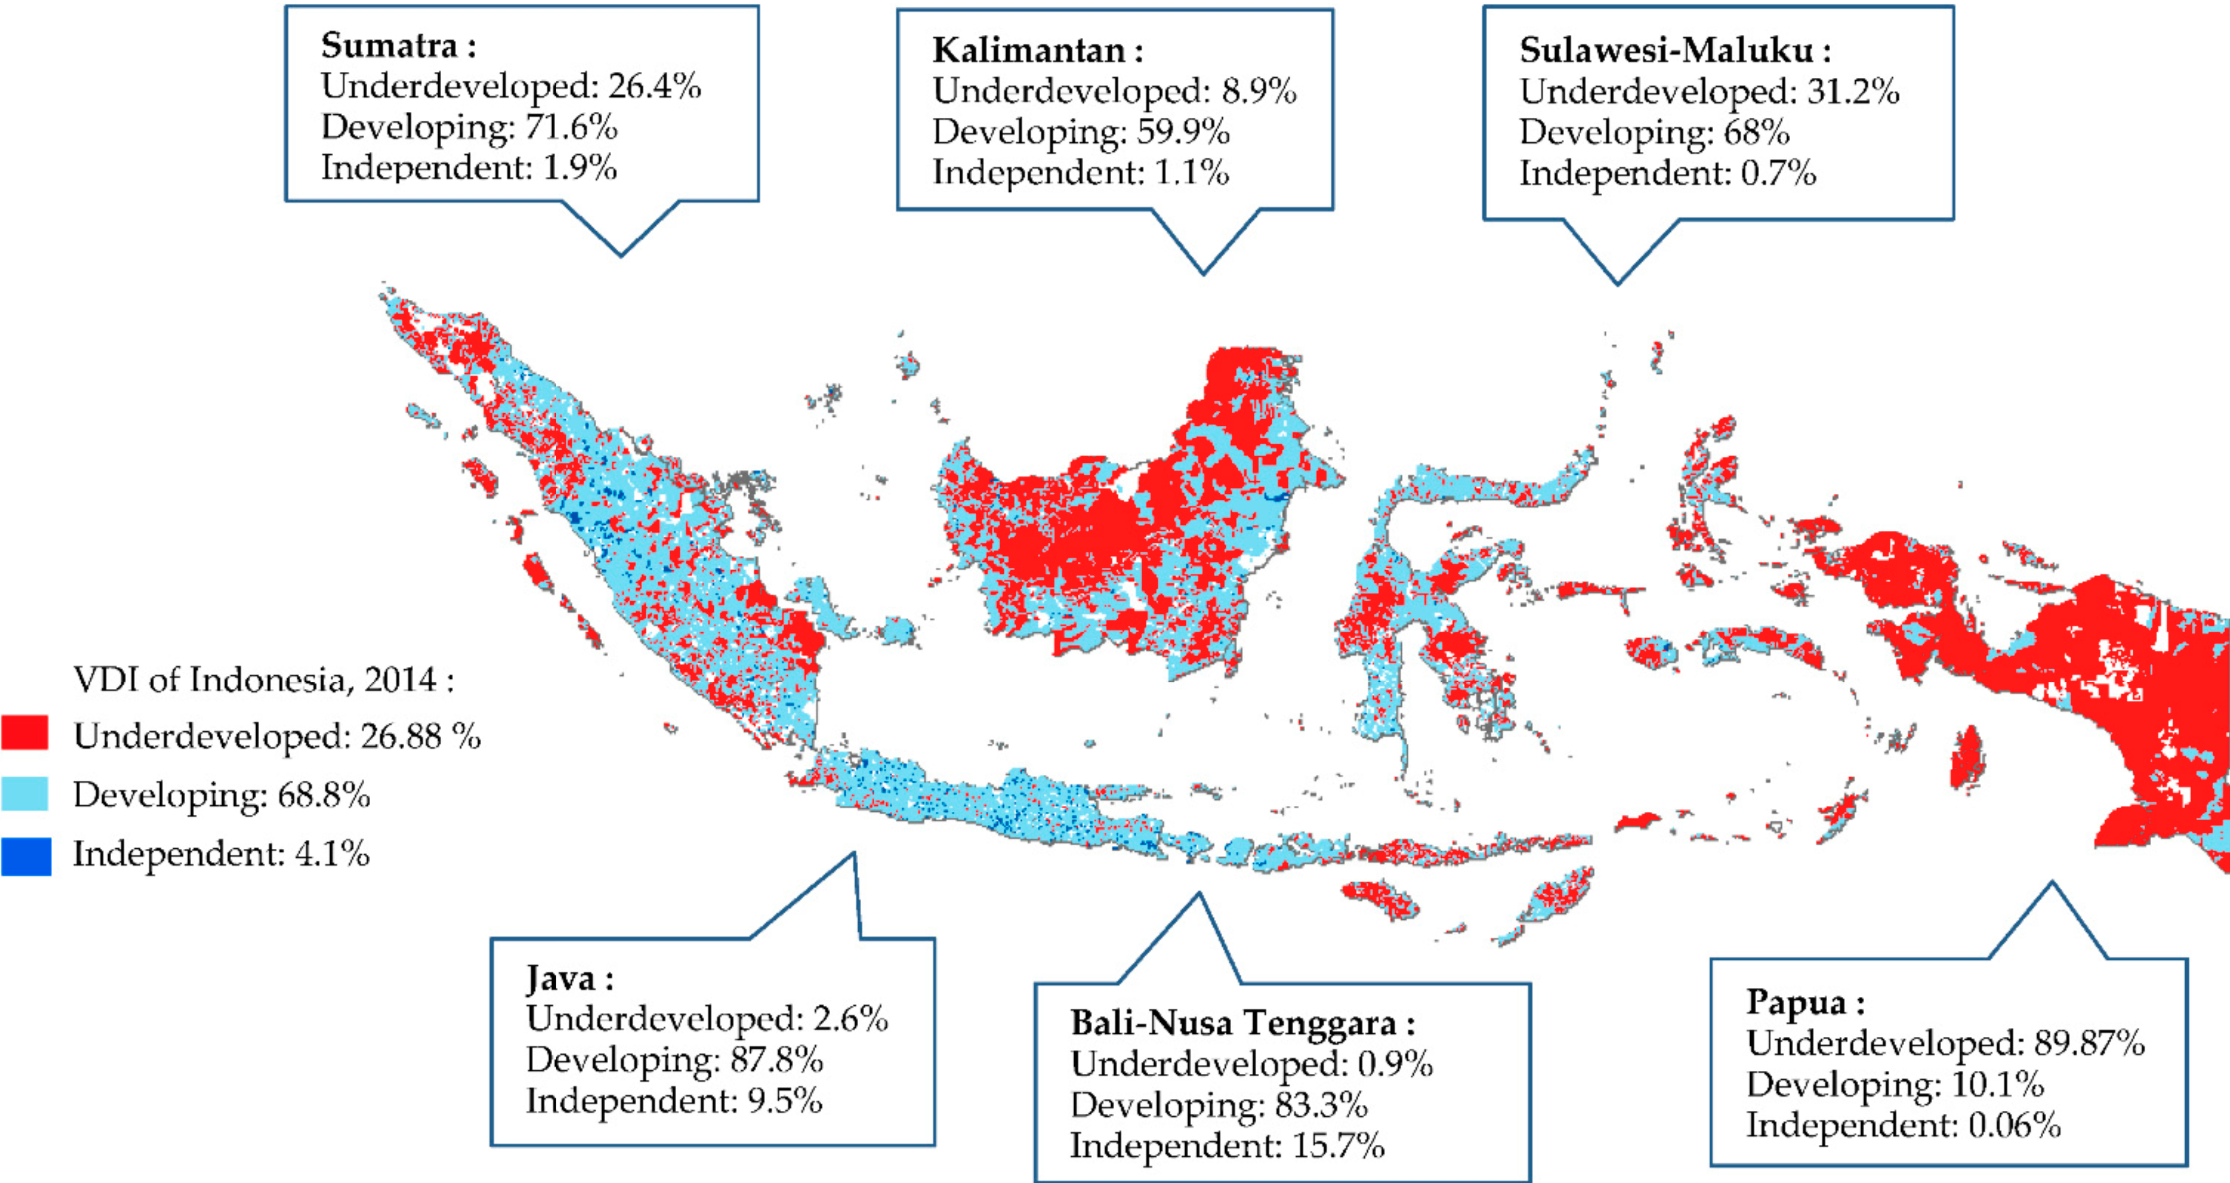
\includegraphics[scale=0.2]{Final_Project/image/vdi2014.png}}\hfill
    \subcaptionbox{Village status in 2018\label{f:panel2}}{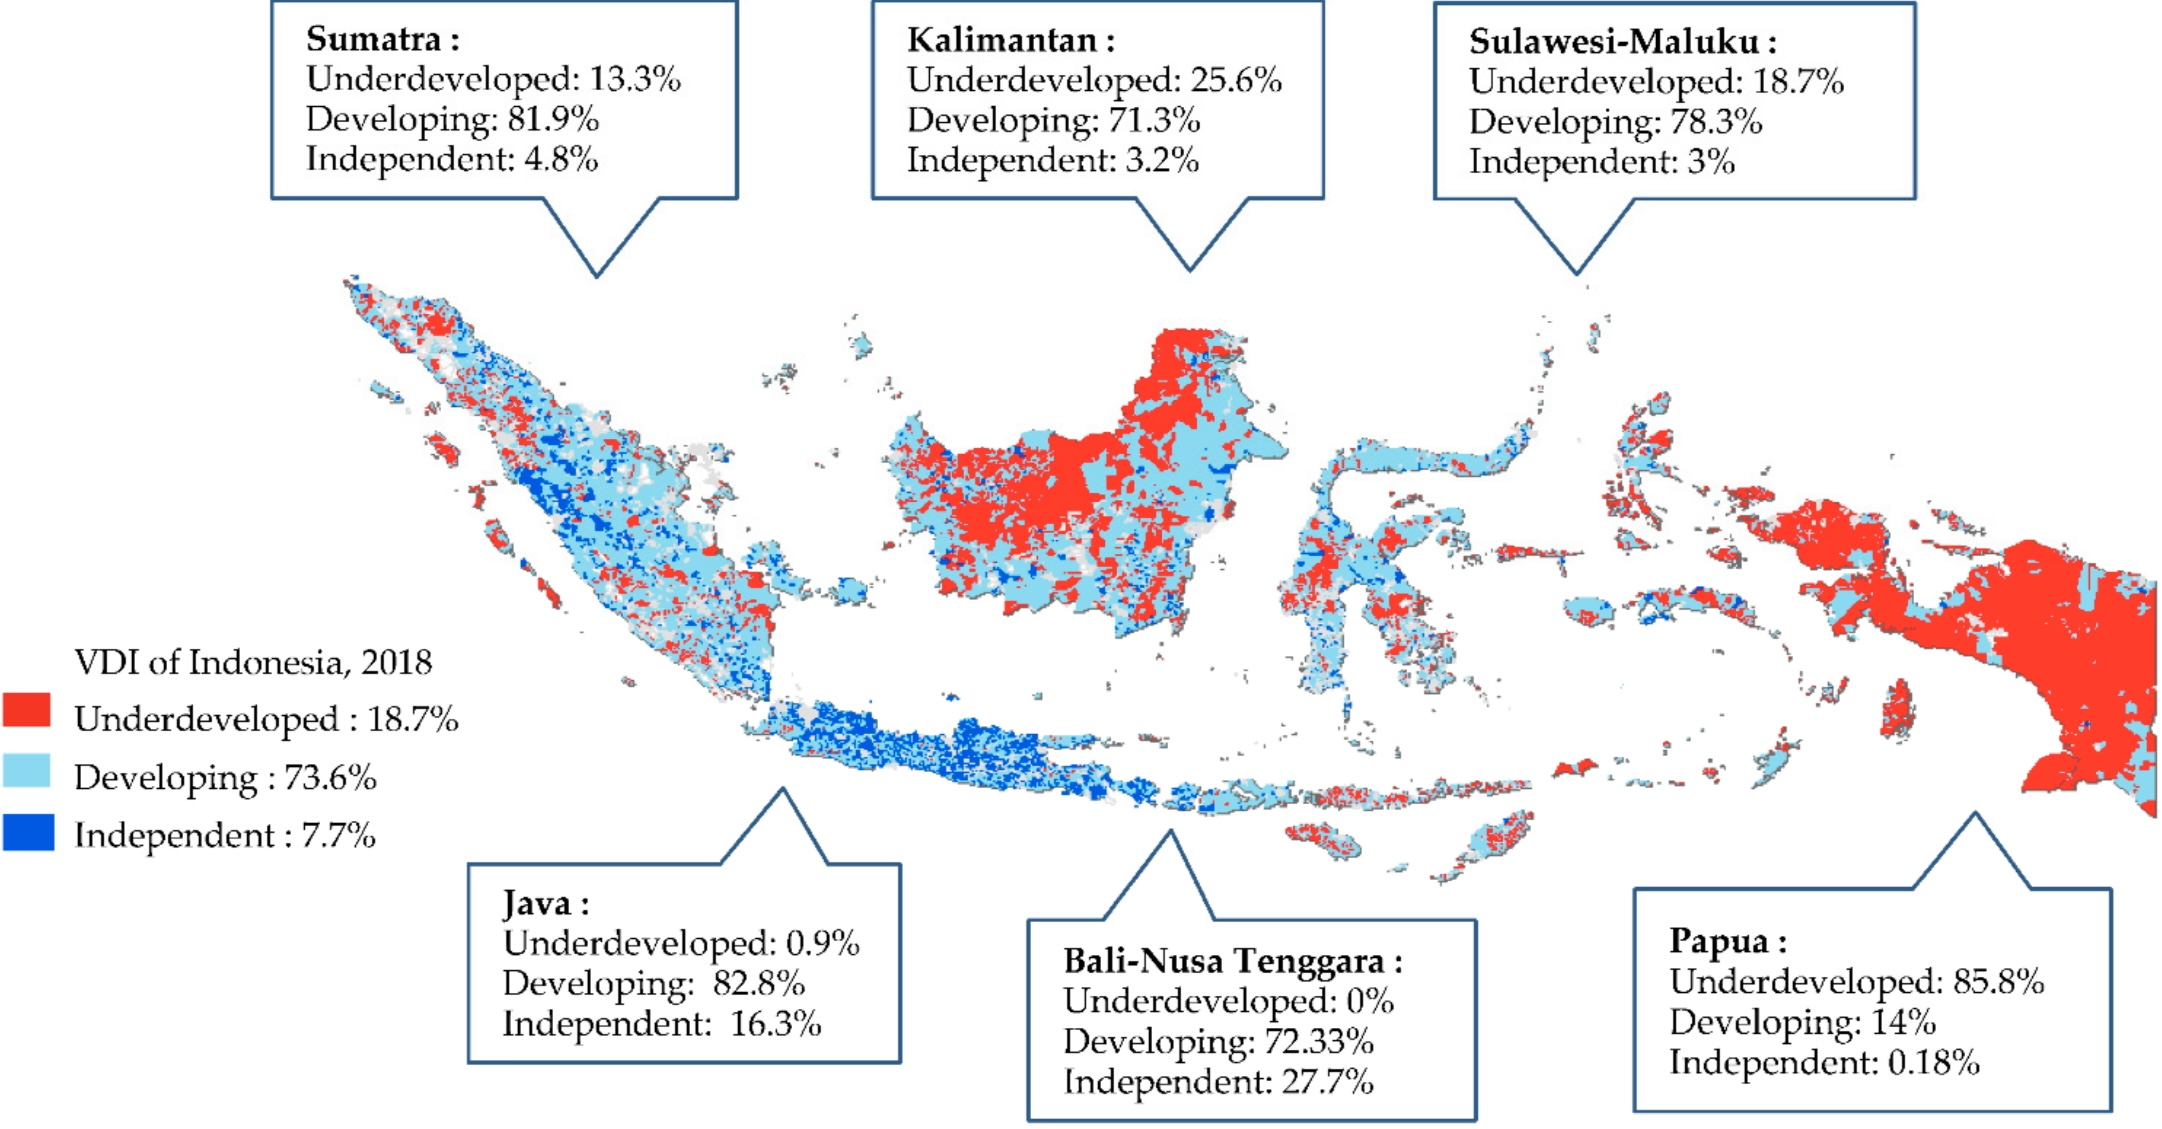
\includegraphics[scale=0.205]{Final_Project/image/vdi2018.jpg}}
    \caption{Indonesia's VDI's status}
    \note{Source: Statistics Indonesia \citet{hartojo_2022}}
    \label{f:graph1}
    \end{figure}
\end{frame}

\section{Empirical Strategy}

\subsection{Measuring rural accessibility with transportation cost}
\begin{frame}
    \begin{itemize}
        \item I measure rural accessibility using the \al{unit transportation cost} (in Rp/km) of each individual village. 
        \item I define unit transportation cost, $y_{it}$, as the \textbf{transportation cost} from the village office to the sub-district office (in thousands Rp), $c_{it}$, divided by the \textbf{distance} from the village office to the sub-district office (in km), $d_{it}$.
        \begin{equation}
        y_{it}=\frac{d_{it}}{c_{it}}    \end{equation}
        
    \end{itemize} 
\end{frame}

\begin{frame}
    \begin{itemize}
        \item The proposed model to estimate is
        \begin{equation}
        y_{it}=+\alpha_i+
        \end{equation}
    \end{itemize}
\end{frame}

\subsection{Data and descriptive statistics}
\begin{frame}
    \begin{itemize}
        \item This study used village in Indonesia as the unit of analysis. 
        \item I obtained the \al{Village Potential Statistics} data for the year 2011, 2014 and 2018 from Indonesia's Central Bureau of Statistics consisting of consecutively 77,961, 82,190, and 83,931 observations.
        \item The survey covers the following module:
        \begin{multicols}{2}
        \begin{itemize}
            \item general information of village,
            \item population and employment, 
            \item housing and environment, 
            \item natural disaster, 
            \item education and health, 
            \item sport and leisure, 
            \item transportation and communication,
            \item land use,
            \item economic activity, 
            \item security, 
            \item \alb{local government}, 
            \item community empowerment, and \item agriculture.
        \end{itemize}
        \end{multicols}
\end{itemize}
\end{frame}
\begin{frame}

   \centering
	\begin{minipage}[b]{0.5\textwidth}

	  \begin{block}{Default}
        Block content.
      \end{block}

      \begin{alertblock}{Alert}
        Block content.
      \end{alertblock}

      \begin{exampleblock}{Example}
        Block content.
      \end{exampleblock}      
      
	\end{minipage}	
\end{frame}


\subsection{Lists}

\begin{frame}
    \begin{columns}[T,onlytextwidth]
    \column{0.33\textwidth}
      \textbf{Items}
      \begin{itemize}
        \item Cats 
        \begin{itemize}
            \item British Shorthair
        \end{itemize}
        \item Dogs \item Birds
      \end{itemize}

    \column{0.33\textwidth}
      \textbf{Enumerations}
      \begin{enumerate}
        \item First 
        \begin{enumerate}
            \item First subpoint
        \end{enumerate}
        \item Second \item Last
      \end{enumerate}

    \column{0.33\textwidth}
      \textbf{Descriptions}
      \begin{description}
        \item[Apples] Yes \item[Oranges] No \item[Grappes] No
      \end{description}
\end{columns}
\end{frame}

\subsection{Table}
\begin{frame}
    \begin{table}
        \caption{Largest cities in the world (source: Wikipedia)}
        \begin{tabular}{@{} lr @{}}
          \toprule
          City & Population\\
          \midrule
          Mexico City & 20,116,842\\
          Shanghai & 19,210,000\\
          Peking & 15,796,450\\
          Istanbul & 14,160,467\\
          \bottomrule
        \end{tabular}
        \hspace*{1cm}
            \setlength\extrarowheight{3pt}
        \begin{tabular}{|lr|}
          \hline
          \rowcolor{primary}\color{white}City & \color{white}Population\\
          \hline
          Mexico City & 20,116,842\\
          Shanghai & 19,210,000\\
          Peking & 15,796,450\\
          Istanbul & 14,160,467\\
          \hline
        \end{tabular}
    \end{table}
\end{frame}

\section{References}
\begin{frame}[allowframebreaks]
    \printbibliography
\end{frame}
\end{document}